\documentclass[../main.tex]{subfiles}

\begin{document}

\section{Sharing the Filesystem}
\label{section:lauxus:sharing}

\par Now that we have seen how LAUXUS works on a local computer, we can dig on the sharing capabilities. As we have seen, the root key is the key material for accessing the Filesystem. Currently, we know that it is sealed on the owner computer. This allows binding the root key to his computer. Indeed, once a material is sealed with SGX, the only party that can unseal it is the SGX instance that sealed it in the first place. This means that we can't just share the sealed version of the root key to other users. As we depicted in Figure \ref{figure:lauxus:approach_crypto}, we need an out of band channel for transmitting the encrypted version of the root key. This is what we will cover in this Section.

\par Before going further, let's remember that currently, every user owns an asymmetric ECC key pair allowing other users to authenticates a message sent by another users (we consider that all the public keys are securely accessible for all the users). This functionality will become handy in our protocol.

\medbreak
\par The sharing protocol is based on the ECDH (Elliptic Curve Diffie-Hellman) particularity. ECDH enables to compute a secret from two key-pairs. Mathematically, if we have two key-pairs: $\mathit{(pk_1, sk_1)}$ and $\mathit{(pk_2, sk_2)}$, a shared secret K can be computed in the following way:
\begin{equation}
    \label{equation:lauxus:ecdh_secret}
    \mathit{K = ECDH\_SECRET(pk_1, sk_2) = ECDH\_SECRET(pk_2, sk_1)}
\end{equation}
With $\mathit{ECDH\_SECRET}$ being a known algorithm in the Elliptic Curve domain.
\par In practice, this means that: two users can securely compute the same secret just by knowing the public key of the other user.


\medbreak
\par As terminology, we will use the same users as in Figure \ref{figure:lauxus:approach_trust}. This means that Alice will share the root key with Carl. In a nutshell, the protocol will be split into 4 phases:
\begin{enumerate}
    \item Alice and Carl will create a message attesting that they are using a valid SGX Enclave. This message will also bind the user to its machine. This message will be called: the \textit{authenticity message}. The \textit{authenticity message} is simply a quote generated by the SGX Enclave in which we add additional information.
    \item Alice will check the authenticity and the validity of the \textit{authenticity message} created by Carl.
    \item Alice will derive a shared secret (this secret is bind to this root key transaction) using the Equation \ref{equation:lauxus:ecdh_secret}. She will then encrypt the root key with this secret and share the result with Carl.
    \item Carl will check the authenticity and the validity of the \textit{authenticity message} created by Alice.
    \item Carl will derive the same shared secret as Alice and will then be able to decrypt the root key before sealing it on his computer.
\end{enumerate}
\par What this all means is that: Alice will encrypt the root key that only Carl can decrypt. This encryption key is unique and binds both users and both user's computers. This means that every time Carl is using a different computer, the protocol must be re-run.
\par To avoid using a third-party server, the above messages will be stored on the remote storage. We this in mind, we created a hidden folder inside the Filesystem containing one directory per user. Each user directory will contain the different message required to add the specific user to the Filesystem.


\subsubsection{Phase 1 - Creating the \textit{authenticity message}}
\begin{figure}[h]
    \centering
    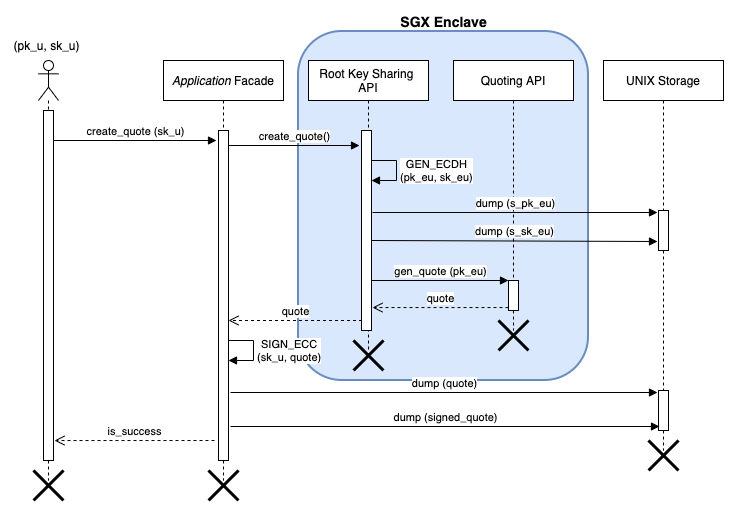
\includegraphics[width=\textwidth]{../../images/lauxus/create_quote}
    
    \caption{Phase 1 Sequence Diagram}
    \label{figure:lauxus:create_quote}
\end{figure}
\par The Figure \ref{figure:lauxus:create_quote} explains the first Phase and is based on the Quoting capability of SGX Enclaves (cfr. Chapter \ref{chapter:theoric}). To bind the user to his computer, we create another key-pair\footnote{pk\_eu stands for the public key of the user U's Enclave - similar notation with the secret key} inside the Enclave and seal them. The quote bears the Enclave public key and the quote is signed using the user private key for authentication.

\subsubsection{Phase 2 - Verifying the \textit{authenticity message}}
\begin{figure}[h]
    \centering
    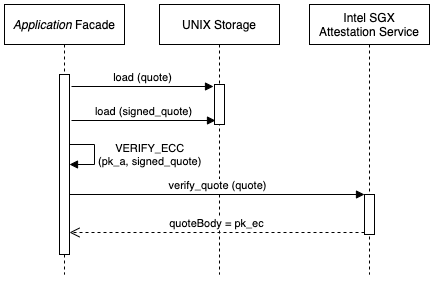
\includegraphics[width=.75\textwidth]{../../images/lauxus/verify_quote}
    
    \caption{Phase 2 Sequence Diagram}
    \label{figure:lauxus:verify_quote}
\end{figure}
\par The Figure \ref{figure:lauxus:verify_quote} explains the second Phase and is based on the remote Intel Attestation Service furnished by Intel (cfr. Chapter \ref{chapter:theoric}). Upon success, the initiator will be sure that this specific user is using a valid SGX Enclave.

\newpage
\subsubsection{Phase 3 - Encrypting the root key for sharing}
\begin{figure}[h]
    \centering
    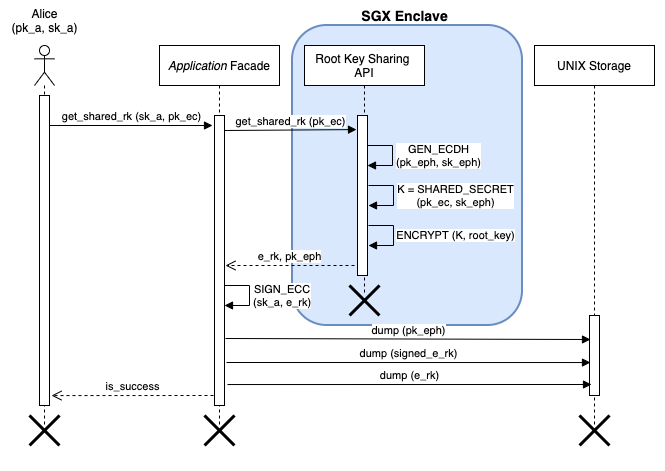
\includegraphics[width=\textwidth]{../../images/lauxus/upload_rk}
    
    \caption{Phase 3 Sequence Diagram}
    \label{figure:lauxus:upload_rk}
\end{figure}
\par The Figure \ref{figure:lauxus:upload_rk} explains the third Phase which is made by the administrator one time for each other user (if the other user never changes his computer). As explained in the Sequence Diagram, Alice creates an ephemeral key-pair\footnote{pk\_eph stands for ephemeral key-pair - similar notation with the secret key}. The encrypted root key is signed with Alice private key to testify authenticity.

\subsubsection{Phase 4 - Decrypting the shared root key}
\begin{figure}[h]
    \centering
    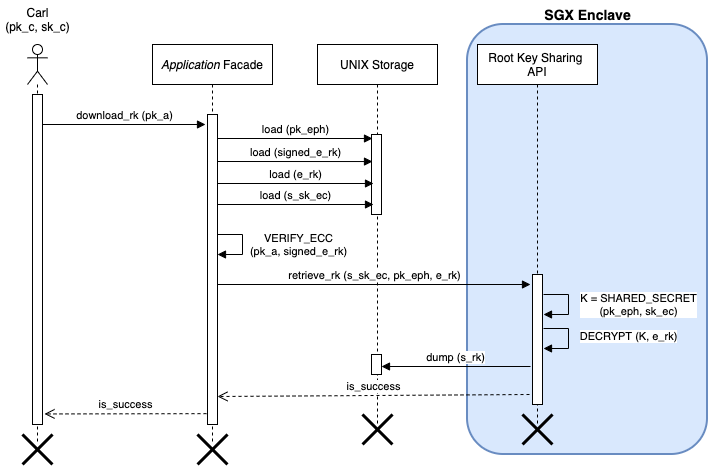
\includegraphics[width=\textwidth]{../../images/lauxus/download_rk}
    
    \caption{Phase 4 Sequence Diagram}
    \label{figure:lauxus:download_rk}
\end{figure}
\par The Figure \ref{figure:lauxus:download_rk} explains the fourth and final Phase which is straightforward knowing the third Phase. We just need to do the opposite operation. The shared secret reconstructed thanks to the ephemeral public key.

\end{document}